\documentclass[a4paper,11pt]{article}

\usepackage[T1]{fontenc}
\usepackage[utf8]{inputenc}
\usepackage{xcolor}
\usepackage{graphicx}
\usepackage{listings}
\usepackage{parskip}
\usepackage{setspace}
\usepackage{float}
\usepackage{tabularx}
\usepackage{hyperref}

\graphicspath{{images/}}

\definecolor{codebackground}{RGB}{247,247,247}
\definecolor{codecomment}{RGB}{0,110,70}
\definecolor{codekeyword}{RGB}{0,70,170}
\definecolor{codestring}{RGB}{160,40,40}

\lstdefinestyle{pythoncode}{
    language=Python,
    backgroundcolor=\color{codebackground},
    basicstyle=\ttfamily\small,
    keywordstyle=\color{codekeyword}\bfseries,
    commentstyle=\color{codecomment}\itshape,
    stringstyle=\color{codestring},
    numbers=left,
    numberstyle=\tiny\color{gray},
    stepnumber=1,
    numbersep=10pt,
    frame=single,
    rulecolor=\color{gray},
    breaklines=true,
    breakatwhitespace=true,
    columns=fullflexible,
    showstringspaces=false,
    tabsize=4,
    captionpos=b,
    aboveskip=1em
}

\lstset{style=pythoncode}
\setlength{\parindent}{0pt}
\setlength{\parskip}{0.5em}
\setstretch{1.05}
\hypersetup{colorlinks=true, urlcolor=blue, linkcolor=black}

\title{Space Robotics -- Assignment 3}

\author{Lucas Plumbohm \\ ...
    \and Elijah Spannenberg \\ ...
    \and Mathis Beissner \\ 26665176}

\date{}

\begin{document}

\setlength{\parindent}{0pt}

\maketitle


\section{Generative AI Disclosure}

Generative AI tools were used to assist with analysing error messages during
the debugging process, creating helper scripts for advanced visual debugging,
formatting this report as a \LaTeX{} document, and
correcting spelling and wording throughout the report.

\section{Statement of Individual Contributions}

\begin{table}[htbp]
    \centering
    \small
    \begin{tabularx}{\textwidth}{@{}l X X X@{}}
        \hline
        Task & Completed? & Team member & Contribution \\
        \hline
        Perception 1 & Yes & Mathis & All \\
        Perception 2 & Yes & Mathis & All \\
        Perception 3 & Yes & Mathis & All \\
        Planning 1 & & & \\
        Planning 2 & & & \\
        Planning 3 & & & \\
        Advanced 1 & & & \\
        Advanced 2 & & & \\
        Advanced 3 & & & \\
        Advanced 4 & & & \\
        Advanced 5 & & & \\
        Advanced 6 & & & \\
        Report writing & & & \\
        Recorded videos & & & \\
        \hline
    \end{tabularx}
\end{table}

\section{Project Overview}
TBA

\section{Implementation}
TBA
% Keep a subsection for each task attempted; remove unattempted task subsections.
% For each task: describe the approach, performance, difficulties and improvements.
% Add relevant code snippets and visual evidence where useful.

% Reusable code-listing template:
% \begin{lstlisting}[caption={Implementation of ...}, label={lst:...}]
% \end{lstlisting}

% Reusable figure template (put image files in images/):
% \begin{figure}[htbp]
%     \centering
%     \includegraphics[width=\linewidth]{filename}
%     \caption{...}
%     \label{fig:...}
% \end{figure}

\newpage

\subsection{Perception 1: Collect an Image Dataset of the Artefacts}
The goal of this task was to collect images of the artefacts to create a dataset
for the subsequent object detection task. The first step was to implement a
manual capture mechanism so that specific, relevant scenes could be selected
and saved. This was achieved by adding a ROS~2 subscriber that listens for
\texttt{std\_msgs/msg/Empty} messages. Publishing one of these messages manually
triggers the \texttt{capture\_callback} method shown below, which sets the
\texttt{capture\_requested\_} flag to \texttt{True} and logs the request.

The system receives new camera images every 0.2 seconds. When a capture has been
requested, the image callback saves the image data and then resets the request
flag. This allows individual scenes to be saved without storing every frame
from the camera stream.

Since depth information could also be useful for the later detection tasks,
the existing image processing was extended by adding a depth image subscriber.
The RGB and depth subscribers were synchronised so that a combined callback
is triggered when corresponding images are available. In addition to the depth
data, a depth image suitable for visual inspection can be saved. A new
configuration file, \texttt{detection\_config.yaml}, was added to specify the
output directories and which image outputs should be saved.

\begin{lstlisting}[caption={Implementation of capture callback}, label={lst:task1}]
    def capture_callback(self, msg):
        self.capture_requested_ = True
        self.get_logger().info('Requesting image capture.')
\end{lstlisting}

\begin{figure}[H]
    \centering
    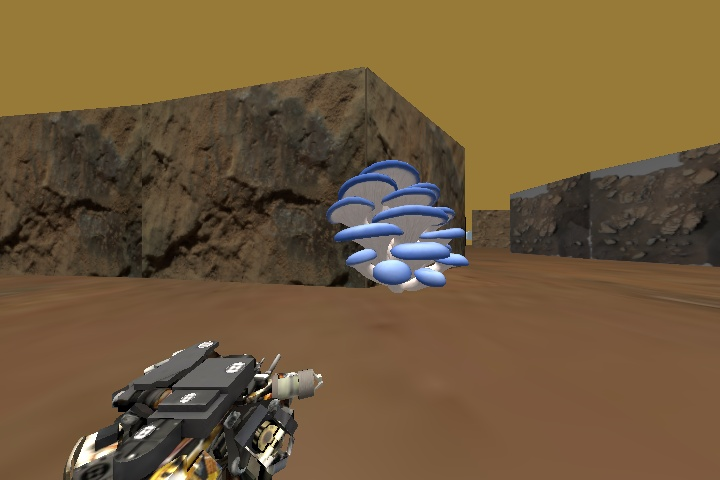
\includegraphics[width=0.42\textwidth]{example_image.jpg}
    \caption{Example image from the collected dataset.}
    \label{fig:example-image}
\end{figure}

\subsection{Perception 2: Detect Artefacts with Computer Vision}
% TF_OLD_DATA ignoring data from the past for frame odom at time 93.450000 according to authority Authority undetectable
% slow inference (longer than 0.2s interval) blocked callback and lead to missing data of some frames
% initally normal ultralytics & inference directly in callback of cave explorer node
% now seperate artifact detection is handled in its own node -> ros_yolo
% also interval reduction of detection possible to improve performance

\subsection{Perception 3: Artefact Localisation and Display}
% using center coordinates of the detected bounding box to estimate the artifact's position.
% center y together with camera fovis used to calc bearing
% artifact distance is calculated by reading depth value at cy & cx, then transforming to distance to robot
% artifact distance & angle are then used to calc artefact position together with robot position
% mistake: used robot position at time of artifact localisation -> after time intensive detection model inference. This led to incorrect artifact positions being calculated, which was especially noticeable while robot was turning
% extended get_pose_2d() function to include timestamp parameter for accurate pose retrieval
% required to make detection callback & get_pose_2d() asynchronous, since i got error message "Lookup would require extrapolation into the future." -> TF message apparently delayed
% to combine different observations of the same artifact to a single estimated position, a Density-Based Spatial Clustering (DBSCAN) algorithm from the scikit-learn library is used.
% DBSCAN groups nearby points into clusters based on a specified distance threshold (eps) and a minimum number of points (min_samples). This helps in reducing noise and improving the accuracy of artifact localization.
% to find the optimal distance threshold, multiple values where tested until a value distance of 3 meters lead to the optimal resulte
% -> In the test run, all observations where clustered perfectly together. Also the "mineral" artefact, consisting of 2 seperate chunks, where clustered perfectly as one artifact, as intended.
\begin{figure}[H]
    \centering
    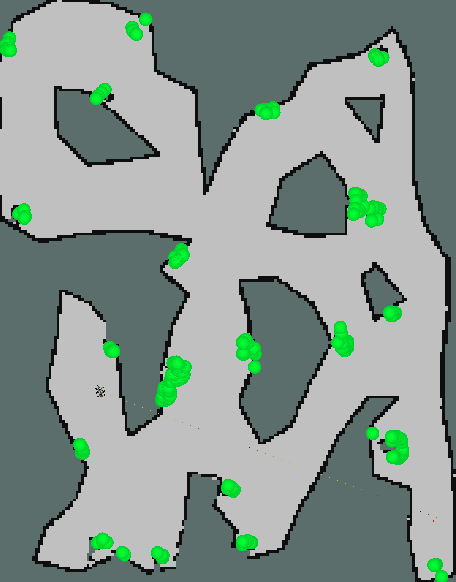
\includegraphics[width=0.48\textwidth]{artifact_localisation.png}
    \hfill
    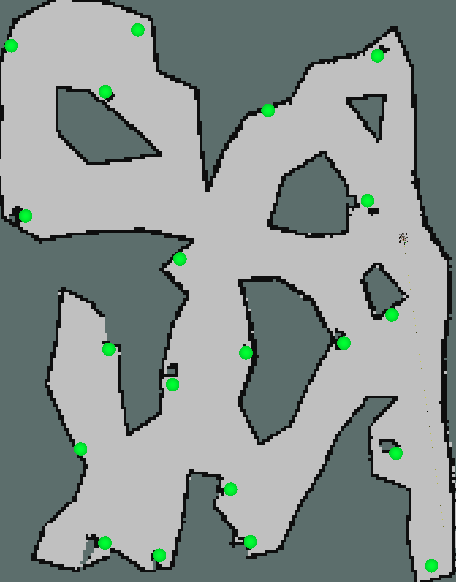
\includegraphics[width=0.48\textwidth]{artifact_localisation_clustered.png}
    \caption{Artefact localisation markers before clustering (left) and after
    DBSCAN clustering (right). Repeated observations are combined into a single
    estimated position for each artefact.}
    \label{fig:artefact-localisation-clustering}
\end{figure}

\subsection{Planning 1: Autonomously Explore the Cave}


\subsection{Planning 2: Close-Range Inspection}


\subsection{Planning 3: Behaviour Switching}


\subsection{Advanced 1: Robust Perception}


\subsection{Advanced 2: Cave Geometry Analysis}


\subsection{Advanced 3: Communication Network Deployment}


\subsection{Advanced 4: Online Roadmap Construction}


\subsection{Advanced 5: Science Tour Planning}


\subsection{Advanced 6: Adaptive Scientific Sampling}


\section{Results}


\section{Reflection on Teamwork}


\end{document}
